\textit{Transformaciones lineales}

\begin{enumerate}[label=\tiny\purple{\faIcon{snowman}}]
  \item Dados $V$ y $W$ dos $K-$espacio vectoriales, una $f: V \to W$ es \textit{transformación lineal}
        si cumple:
        \begin{itemize}
          \item $f(v_1 + v_2) = f(v_1) + f(v_2) \quad \paratodo v, w \en V$
          \item $f(\alpha \accion v_1) = \alpha \cdot f(v_1) \quad \paratodo \alpha \en K, v \en V$
        \end{itemize}
  \item $f: K^n \to K^m$ si transformo:
        $$
          f(x_1, \cdots, x_n) =
          f\Big(\sumatoria{k=1}{n} x_i \accion \ub{e_i}{\en K^{n \times 1}}\Big) \igual{TL}
          \sumatoria{k=1}{n} x_i \cdot \ub{f(e_i)}{\en K^{m \times 1}} =
          \ub{\matriz{c|c|c}{
              f(e_1) & \cdots & f(e_n)
            }
          }{A \en K^{m \times n}}
          \cdot
          \matriz{c}{
            x_i\\
            \vdots\\
            x_n
          }
          = \ub{A \cdot x}{ \en K^{m \times 1}}
        $$

  \item \textit{Matriz de una transformación lineal:}

        Dados $V$ y $W$ dos $K-$espacios vectoriales y
        $f: V \to W$ una t.l. Sean $B = \set{v_1, \cdots, v_2}$ base de $V$ y $B' = \set{w_1, \cdots, w_m}$
        se llama matriz de la transformación lineal de la base $B$
        en la base $B'$ a aquella matriz $[f]_{BB'}$ que satisface:
        $$
          [f]_{BB'} [v]_B = [f(v)]_{B'} \quad \paratodo v \en V
        $$
\end{enumerate}

\textit{Aritmética de punto flotante:}
\begin{enumerate}[label=\tiny\purple{\faIcon{snowman}}]
  \item
        \textit{Escribir $0.25$ en base $10$}:

        Base 10 es obviamente nuestra base favorita:
        $$
          \llave{rcl}{
            0.25 \cdot 10 & = & 2 + 0.5\\
            0.5  \cdot 10 & = & 5 + 0\\
            0 \cdot 10 & = & 0 + 0
          }
          \to
          (0.25)_{10} =
          (2 \cdot 10^{-1} +
          5 \cdot 10^{-2} +
          0 \cdot 10^{-3} + 0)_{10}
          = 0.25
        $$

        \textit{Escribir $0.25$ en base $2$}:
        $$
          \llave{rcl}{
            0.25 \cdot 2 & = & 0 + 0.5\\
            0.5  \cdot 2 & = & 1 + 0\\
            0 \cdot 2 & = & 0 + 0
          }
          \to
          (0.25)_2 =
          (0 \cdot 2^{-1} +
          1 \cdot 2^{-2} +
          0 \cdot 2^{-3} + 0)_2
          = 0.01
        $$

        \textit{Escribir $0.3$ en base $2$}:
        $$
          \llave{rcl}{
            0.3 \cdot 2 & = & \magenta{0} + 0.6\\
            0.6 \cdot 2 & = & \magenta{1} + 0.2\\ \rowcolor{Cerulean!10}
            0.2 \cdot 2 & = & \magenta{0} + 0.4\\
            0.4 \cdot 2 & = & \magenta{0} + 0.8\\
            0.8 \cdot 2 & = & \magenta{1} + 0.6\\
            0.6 \cdot 2 & = & \magenta{1} + 0.2\\ \rowcolor{Cerulean!10}
            0.2 \cdot 2 & = & \magenta{0} + 0.4\\
            0.4 \cdot 2 & = & \magenta{0} + 0.8\\
            0.8 \cdot 2 & = & \magenta{1} + 0.6\\
            \vdots & = & \vdots
          }
          \scriptstyle
          \to
          (0.3)_{2} =
          (
          \magenta{0} \cdot 2^{-1} +
          \magenta{1} \cdot 2^{-2} +
          \magenta{0} \cdot 2^{-3} +
          \magenta{0} \cdot 2^{-4} +
          \magenta{1} \cdot 2^{-5} +
          \magenta{1} \cdot 2^{-6} +
          \magenta{0} \cdot 2^{-7} +
          \magenta{0} \cdot 2^{-8} +
          \magenta{1} \cdot 2^{-9} +
          \magenta{1} \cdot 2^{-10} +
          \magenta{0} \cdot 2^{-11} +
          \magenta{0} \cdot 2^{-12}
          \cdots )_2=
          0.01\overline{0011}
        $$
        Para escribir al $0.3$ en base 2 voy a necesitar infinitos números en la \textit{mantisa}, la máquina no puede y ahí aparecen
        los errores de \textit{redondeo} o \textit{truncamiento}.

        \bigskip
        \textit{Errores:}

        Tengo que un \textit{número de máquina}, número posta que la máquina representa, con la notación \textit{mantisa}, \textit{exponente}:
        $$
          \begin{array}{l}
            \text{En base 10} \to x = 0,a_1a_2a_3 \ldots a_m \cdot 10^{exp}  \text{ con } 0 \leq a_i \leq 9 (a_1 \distinto 0) \\
            \text{En base 2} \to x = 0,a_1a_2a_3 \ldots a_m \cdot 2^{exp}  \text{ con } 0 \leq a_i \leq 1  (a_1 \distinto 0)
          \end{array}
        $$

        Por ejemplo si $m = 3 \entonces x = 0,a_1a_2a_3 \cdot 2^{exp}$.
        Para cada valor de $exp$ voy a tener un total de $\ua{1}{a_1} \cdot \ua{2}{a_2} \cdot \ua{2}{a_3} = 4$ posibles valores de máquina.
        La separación entre 2 valores $x_1$ y $x_2$ consecutivos es de $2^m$, por eso para órdenes grandes la separación entre un número y otro
        es mayor.

        Si el número real, real que quiero es $x = 0.3$, la máquina no puede representarlo de forma exacta. Puedo acotar el error en forma absoluta como:
        $$
          |x - x^*| \leq \frac{1}{2} \frac{1}{2^m}\cdot 2^{exp}
        $$
        Y en forma relativa como:
        $$
          \frac{|x - x^*|}{|x|} \leq 5 \cdot 2^{-m}
        $$
\end{enumerate}

\textit{Deducción matriz de rotación 2d {\tiny (ponele)}:}

Quiero que:
$$
  \matriz{cc}{
    a & b \\
    c & d
  }
  \cdot
  \matriz{c}{
    u\\
    v
  }
  =
  \ub{
    \matriz{c}{
      a\\
      c
    }
    \cdot u_0
  }{\llamada1 }
  +
  \ub{
    \matriz{c}{
      b\\
      d
    }
    \cdot v_0
  }{\llamada2}
  =
  \matriz{c}{
    u_{\theta}\\
    v_{\theta}
  }
$$

En el gráfico veo lo que quiero lograr.

$$
  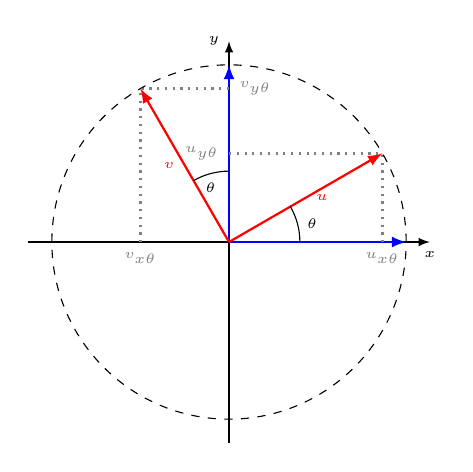
\begin{tikzpicture}[scale=1.5, every node/.style={font=\tiny}]
    \draw[-latex] (-1.7,0) -- (1.7,0) node[below] {$x$};
    \draw[-latex] (0,-1.7) -- (0,1.7) node[left] {$y$};

    \draw[-latex, thick, blue] (0,0) -- (1.5,0);
    \draw[-latex, thick, blue] (0,0) -- (0,1.5);

    \draw[-latex, thick, red] (0,0) -- ({1.5*cos(30)},{1.5*sin(30)}) node[midway, right] {$u$};
    \draw[dotted, thick, gray] (0,{1.5*sin(30)}) node[left] {$u_{y\theta}$} -- ({1.5*cos(30)},{1.5*sin(30)}) -- ({1.5*cos(30)},0) node[below] {$u_{x\theta}$};

    \draw[-latex, thick, red] (0,0) -- ({-1.5*sin(30)},{1.5*cos(30)}) node[midway, left] {$v$};
    \draw[dotted, thick, gray] (0,{1.5*cos(30)}) node[right] {$v_{y\theta}$} -- ({-1.5*sin(30)},{1.5*cos(30)}) -- ({-1.5*sin(30)},0) node[below] {$v_{x\theta}$};

    \draw (0.6,0) arc (0:30:0.6) node[midway, right] {$\theta$};
    \draw (0,0.6) arc (90:120:0.6) node[midway, below] {$\theta$};

    \draw[dashed, black] (0,0) circle (1.5);
    % \draw[-latex, thick, brown] (1.2,0.1) arc (5:40:1.2) node[midway, above right] {tuqui};
  \end{tikzpicture}
$$

Entre el gráfico y $\llamada1$:
$$
  \matriz{c}{
    a\\
    c
  }
  \cdot u_0
  =
  \matriz{c}{
    u_{x\theta} \\
    u_{y\theta}
  }
  \ua{\igual{\red{!}}}{\text{\tiny sohcatoa}}
  \matriz{c}{
    u_0 \cdot \cos(\theta) \\
    u_0 \cdot \sin(\theta) \\
  }
  \sii
  \matriz{c}{
    a\\
    c
  }
  =
  \matriz{c}{
    \cos(\theta) \\
    \sin(\theta)
  }
$$
Entre el gráfico y $\llamada2$:
$$
  \matriz{c}{
    b\\
    d
  }
  \cdot v_0
  =
  \matriz{c}{
    v_{x\theta} \\
    v_{y\theta}
  }
  \ua{\igual{\red{!}}}{\text{\tiny sohcatoa}}
  \matriz{c}{
    - v_0 \cdot \sin(\theta) \\
    v_0 \cdot \cos(\theta)
  }
  \sii
  \matriz{c}{
    b\\
    d
  }
  =
  \matriz{c}{
    -\sin(\theta) \\
    \cos(\theta)
  }
$$
Juntando esos resultados:
$$
  R_{\theta}
  =
  \matriz{cc}{
    a & b \\
    c & d
  }
  =
  \matriz{cc}{
    \cos(\theta) & -\sin(\theta) \\
    \sin(\theta) & \cos(\theta)
  }
$$
